%%%%%%%%%%%%%%%%%%%%%%%%%%%%%%%%%%%%%%%%%%%%%%%%%%%%%%%%%%%%%%%%%%%%%%%%%%%%%%%%
%2345678901234567890123456789012345678901234567890123456789012345678901234567890
%        1         2         3         4         5         6         7         8

\documentclass[letterpaper, 10 pt, conference]{ieeeconf}  % Comment this line out
                                                          % if you need a4paper
%\documentclass[a4paper, 10pt, conference]{ieeeconf}      % Use this line for a4
                                                          % paper

\IEEEoverridecommandlockouts                              % This command is only
                                                          % needed if you want to
                                                          % use the \thanks command
\overrideIEEEmargins
% See the \addtolength command later in the file to balance the column lengths
% on the last page of the document



% The following packages can be found on http:\\www.ctan.org
%\usepackage{graphics} % for pdf, bitmapped graphics files
%\usepackage{epsfig} % for postscript graphics files
\usepackage{mathptmx} % assumes new font selection scheme installed
%\usepackage{times} % assumes new font selection scheme installed
\usepackage{amsmath} % assumes amsmath package installed
\usepackage{amssymb}  % assumes amsmath package installed
\usepackage{float}
\usepackage{array}
\usepackage[spanish]{babel}
\usepackage{comment}
\usepackage{graphicx}


\title{\LARGE \bf
An\'alisis del crimen en La Haya, Pa\'ises Bajos: \\
Aplicaci\'on de Teor\'ia de Grafos 
}

%\author{ \parbox{3 in}{\centering Huibert Kwakernaak*
%         \thanks{*Use the $\backslash$thanks command to put information here}\\
%         Faculty of Electrical Engineering, Mathematics and Computer Science\\
%         University of Twente\\
%         7500 AE Enschede, The Netherlands\\
%         {\tt\small h.kwakernaak@autsubmit.com}}
%         \hspace*{ 0.5 in}
%         \parbox{3 in}{ \centering Pradeep Misra**
%         \thanks{**The footnote marks may be inserted manually}\\
%        Department of Electrical Engineering \\
%         Wright State University\\
%         Dayton, OH 45435, USA\\
%         {\tt\small pmisra@cs.wright.edu}}
%}

\author{Pedro Vladimir Hern\'andez Serrano, Jos\'e Alfredo M\'endez Barrera y Elisa Hern\'andez Rodr\'iguez % <-this % stops a space
}


\begin{document}



\maketitle
\thispagestyle{empty}
\pagestyle{empty}


%%%%%%%%%%%%%%%%%%%%%%%%%%%%%%%%%%%%%%%%%%%%%%%%%%%%%%%%%%%%%%%%%%%%%%%%%%%%%%%%
\begin{abstract}

En el presente documento se analiz\'o el crimen en la Haya a trav\'es de t\'ecnicas anal\'iticas utilizadas en teor\'ia de grafos. El objetivo principal del estudio fue el de caracterizar a las colonias de La Haya, Pa\'ises Bajos para conocer los flujos de reubicaci\'on de personas y hacer un primer acercamiento a su relaci\'on con el crimen. El análisis fue realizado con ayuda de Neo4j y Cypher Query Language. Con el uso de dichas herramientas y la exploraci\'on de datos se encontr\'o primeros indicios para explicar el cambio de residencia de las personas en colonias con m\'as interacciones con respecto a las dem\'as as\'i como la medida de criminalidad juega un papel indispensable pero no concluyente. 

\end{abstract}

%%%%%%%%%%%%%%%%%%%%%%%%%%%%%%%%%%%%%%%%%%%%%%%%%%%%%%%%%%%%%%%%%%%%%%%%%%%%%%%%
\section{INTRODUCI\'ON}
\vspace{2mm}
La descomposi\'on de las colonias conlleva consecuencias que afectan el nivel de vida de las personas e indirectamente aquejan a colonias cercanas. Una de las situaciones m\'as frecuentes por las cuales surge dicha descomposici\'on  son la delincuencia y el miedo o percepci\'on hacia la delincuencia, lo que puede desencadenar la reubicaci\'on como una medida de precauci\'on. En este contexto, surgen preguntas fundamentales;

\begin{itemize}
\item \textquestiondown Cu\'ales son las colonias que m\'as gente abandona?
\item \textquestiondown Cu\'ales son las colonias donde se reubica m\'as la gente?
\item \textquestiondown Cu\'ales son las colonias con mayor delincuencia?
\item \textquestiondown Cu\'ales son los distritos que tienen m\'as influencia?
\item \textquestiondown Las personas se reubican en sitios con menor grado de delincuencia?
\end{itemize}

%%%%%%%%%%%%%%%%%%%%%%%%%%%%%%%%%%%%%%%%%%%%%%%%%%%%%%%%%%%%%%%%%%%%%%%%%%%%%%%%
\section{DATOS}
\vspace{2mm}

\subsection{Descripci\'on de los datos}

Para este an\'alisis se contruy\'o una base de datos de panel, considerando  las variables que pueden estar ligadas con la reubicaci\'on (migraci\'on interna). Dicha base de datos se compone de las 114 colonias que constituyen la Haya en los Pa\'ises Bajos desde 2003 hasta 2009 (las cifras se han extra\'ido de los documentos oficiales recopilados por el municipio de La Haya (Den Haag in cijfers, DHIC). La base de datos incluye los siguientes grupos variables: 
\vspace{2mm}
\begin{enumerate}
\item \textit{\textbf{Flujos de reubicaci\'on}}
Los fujos de reubicaci\'on incluyen 114 colonias en la Haya, est\'a informaci\'on est\'a disponible para 7 a\~nos (2003-2009).
\vspace{2mm}
\item \textit{\textbf{Crimen}}
Estas variables se refieren a la informaci\'on reportada al Departamento de Polic\'ia. Por su naturaleza, las variables se dividieron en en dos grupos: 
\begin{itemize}
\item Crimen cometido directamente a personas (o crimen por violencia). Este tipo crimen incluye amenazas, maltrato y robo en las calles.
\item Crimen a propiedad, el cual se compone po las variables robo de autom\'ovil, robo de objetos del autom\'ovil, robo en compañ\'ias o negocios, robo de mercanc\'ia en tiendas, robo de cartera y robo en casa-habitaci\'on.
\end{itemize}
\vspace{2mm}
\item \textit{\textbf{Colonias}}
Las colonias que componen a la Haya.
\vspace{2mm}
\item \textit{\textbf{Criminales}}
Esta variable se refiere al n\'umero de criminales ubicados en cada colonia.
\vspace{2mm}
\item \textit{\textbf{Distancia}}
Corresponde a la distancia entre el centroide de la colonia i a la colonia j.
\end{enumerate}
\subsection{Descripci\'on del Grafo}
El grafo incluye 3 tipos de nodos vinculados con los datos anteriormente descritos. La composici\'on del grafo es de  804 nodos y 80,981 aristas.

\def\arraystretch{1.5} %distancia entre las filas
\begin{table}[H]
\centering
\caption{\textbf{Nodos}}
\footnotesize
\centering
\begin{tabular}{p{1.3cm} p{2.6cm} p{3.5cm}}
\textbf{Nombre} &  \textbf{Nombre en el Grafo} & \textbf{Atributos}\\
\hline
\hline 
\textit{A\~no} & year &\\
\textit{Colonia} & zona & no. criminales, no. de crimenes nombre\\
\textit{Distrito} & regi\'on & nombre
\end{tabular}
\label{tab:t_nodos}
\end{table}

Los nodos de color verde corresponden al a\~no, los amarillos a las colonia y los morados a los distritos.

De la misma manera, fueron tambi\'en definidas 3 tipos de relaciones. Dichas definiciones pueden observarse claramente en la Figura 1

\def\arraystretch{1.5} %distancia entre las filas
\begin{table}[H]
\centering
\caption{\textbf{Relaciones}}
\footnotesize
\centering
\begin{tabular}{p{1cm} p{1cm} p{2.5cm} p{2.5cm}}
\textbf{Nombre} &  \textbf{Grafo} & \textbf{Descripci\'on} & \textbf{Atributos}\\
\hline
\hline 
\textit{Pertenece} & belong & la colonia pertenece a un distrito & \\
\textit{Crimen} & crime & el distrito tiene un n\'umero de crimenes por año & crimenes en el origen, crimenes en el destino\\
\textit{Flujos} & move to & la colonia i tiene reubicaciones en la colonia j & no. personas que se reubicaron (peso de la arista)
\end{tabular}
\label{tab:t_relaciones}
\end{table}

\begin{figure}[ht]
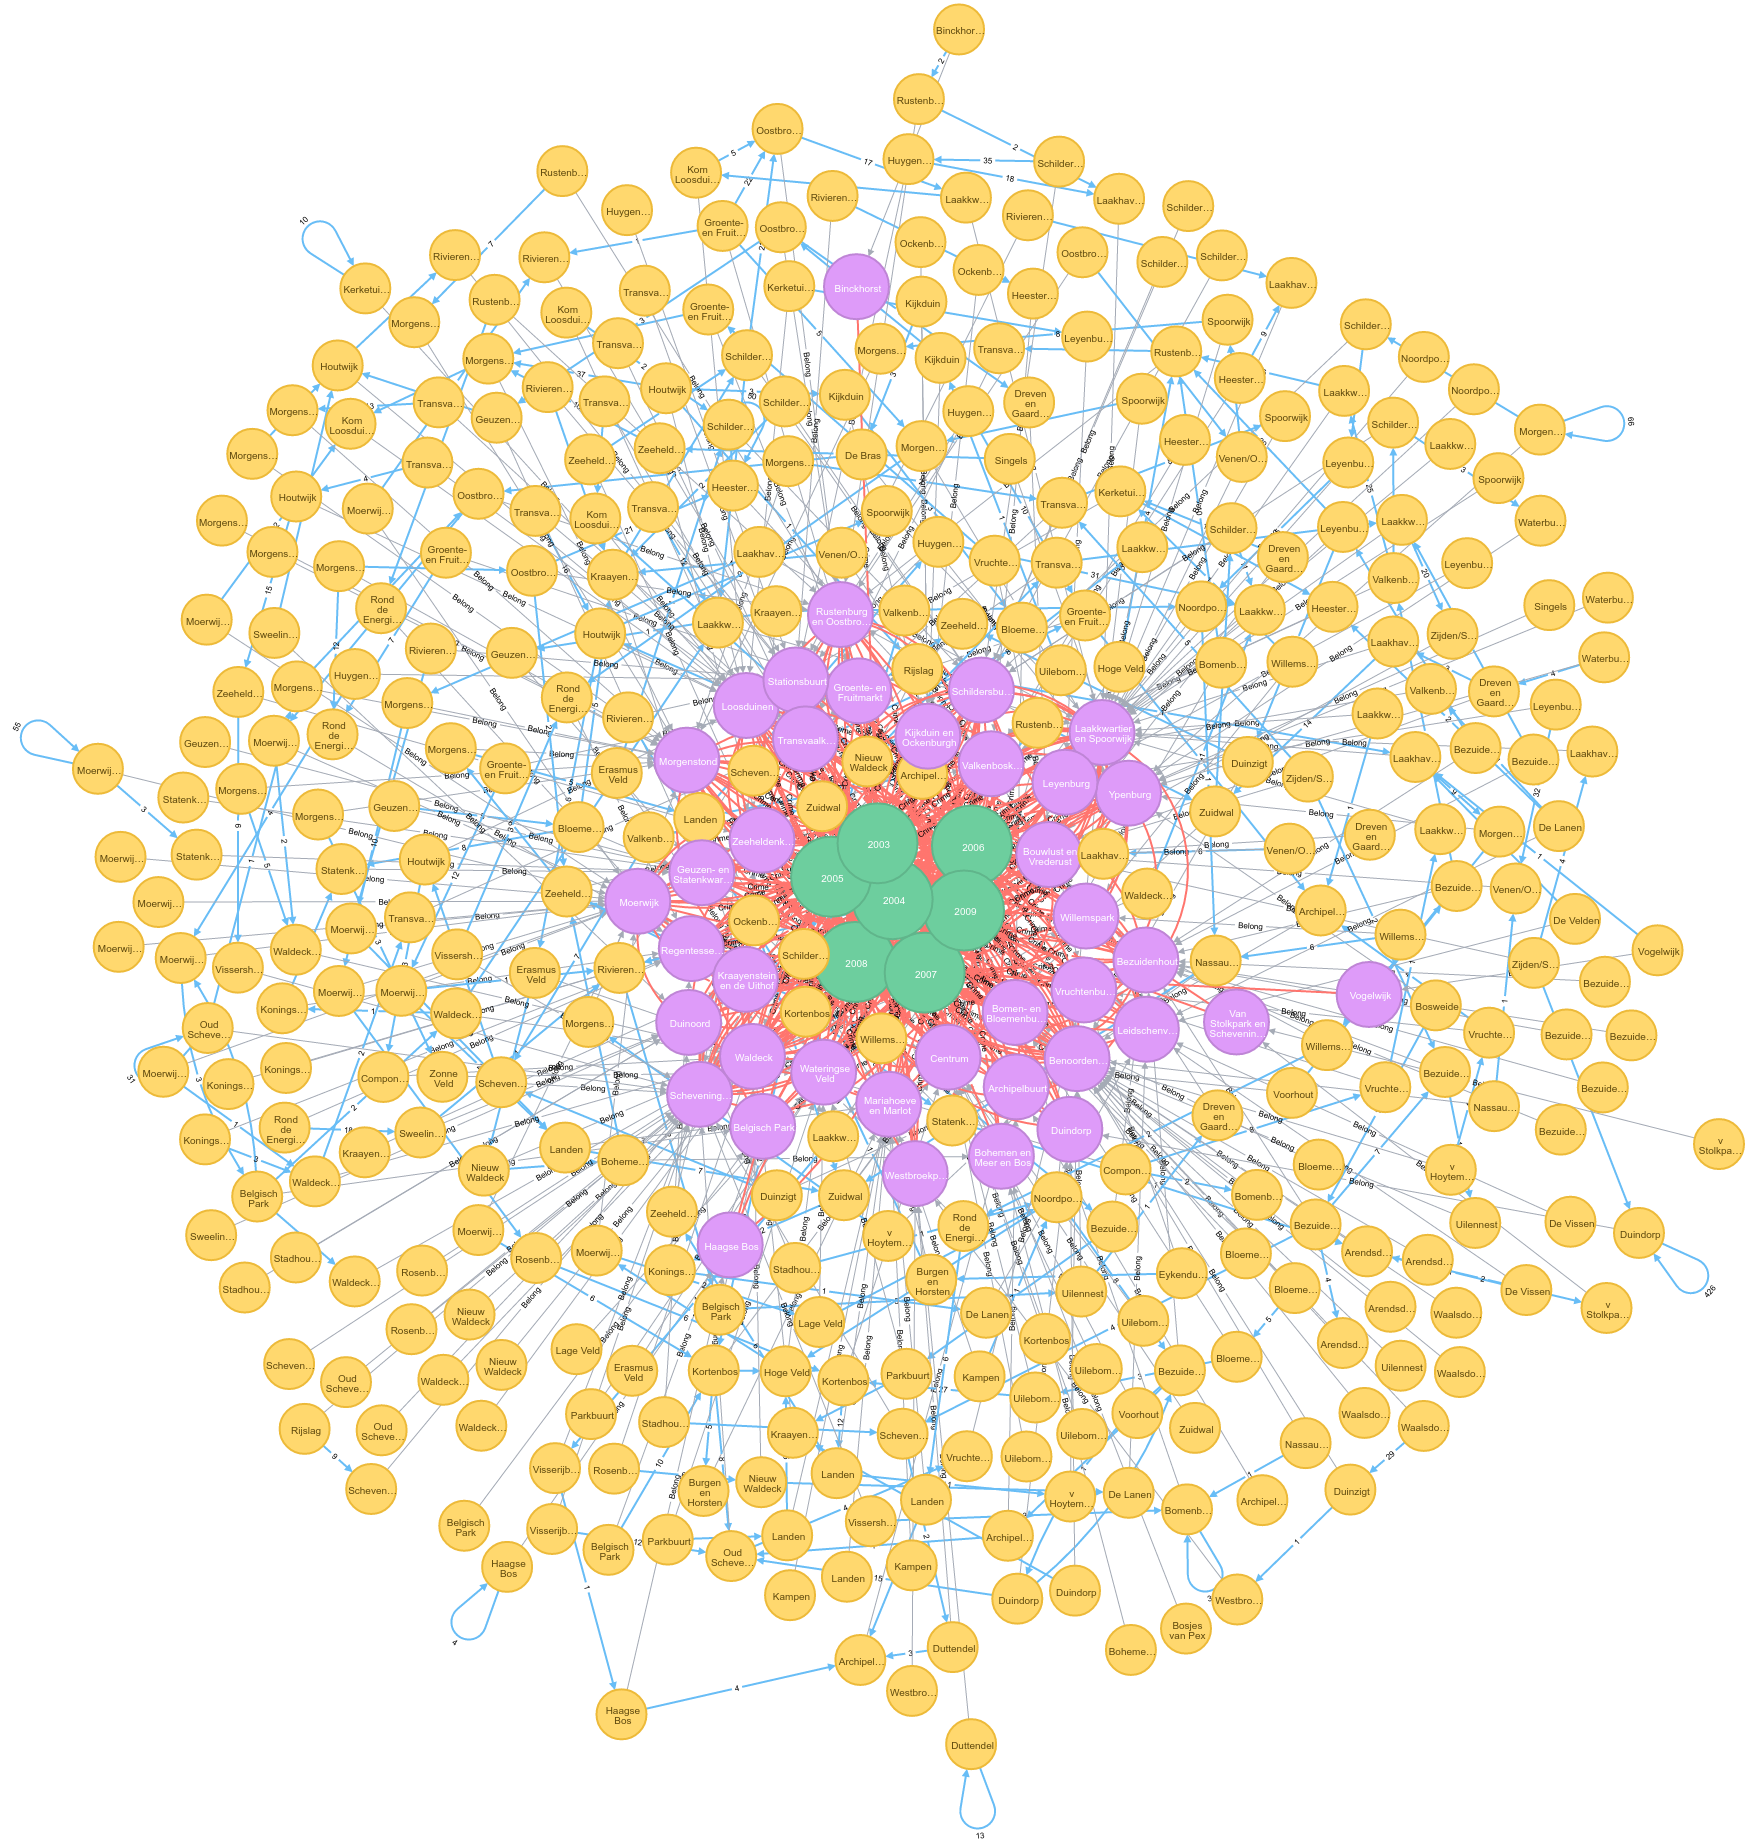
\includegraphics[width=9cm]{graph_all.png}
\caption{Representaci\'on gr\'afica de los datos}
\label{tab:grafo}
\end{figure}

\section{METODOLOG\'IA}
\vspace{2mm}

\subsection{Herramientas}

El análisis se realiz\'o a trav\'es de Neo4j, utilizando Cypher Query Language. La base de datos orientada a grafos $Neo4j$ posibilit\'o la visualizaci\'on de los datos en forma de nodos y relaciones. CQL por su parte permiti\'o la consulta y actualizaci\'on gr\'afica.

\subsection{Conceptos}
Con el fin de realizar un an\'alisis descriptivo de los datos y contestar las preguntas objetivo fueron utilizados algunos conceptos fundamentales encontrados en la Teor\'ia de grafos.

Primero, para la descripci\'on del grafo se contaron el n\'umero de \textbf{nodos} $804$ as\'i como el n\'umero de \textbf{aristas} $80,981$, los cuales marcan las relaciones existentes en la base de datos. Posteriormente, fue realizada una exploraci\'on m\'as profunda por medio del c\'alculo de los \textbf{in-grados}, \textbf{ex-grados} y \textbf{total de grados}. Esto \'ultimo permiti\'o conocer las colonias con m\'as relaciones.

Asimismo, se calcul\'o el \textbf{di\'ametro} del grafo con la finalidad de conocer la m\'axima \textbf{excentricidad} respecto a los nodos (camino m\'as largo) y as\'i el camino de m\'aximo peso tomando en cuenta las relaciones anteriormente descritas.

Finalmente, fue implementado el \textbf{algoritmo Dijkstra}, que consiste en encontrar los caminos m\'as cortos a partir de un origen. Este algor\'itmo result\'o en las colonias a las que es m\'as sencillo reubicarse.

\section{RESULTADOS}
\vspace{2mm}
Los nodos principales son los correspondientes a las colonias, ya que incluyen m\'as relaciones y permitir\'a contestar las preguntas objetivo de este an\'alisis. Considerando lo anterior se examinaron las caracter\'isticas de dichos nodos. El ex-grado por un lado indica que en $111$ colonias tuvieron habitantes que se reubicaron, mostrando $41,063$ interacciones. El in-grado muestra que solo en 4 colonias no hubo flujo poblacional, las cuales podr\'iamos clasificarlas como nodos $hoja$

\def\arraystretch{1.5} %distancia entre las filas
\begin{table}[H]
\centering
\caption{\textbf{No. de colonias de donde los habitantes se reubican}}
\footnotesize
\centering
\begin{tabular}{p{3cm} p{1.5cm} p{1.5cm}}
\textbf{Colonia} &  \textbf{Ex-grado} & \textbf{Ranking}\\
\hline
\hline 
\textit{Zeeheldenkwartier} & 651 & 1 \\
\textit{Valkenboskwartier} & 633 & 2 \\
\textit{Kortenbos} & 625 & 3 \\
\textit{Leyenburg} & 622 & 4 \\
\textit{Koningsplein eo} & 606 & 5 \\
\textit{Rietbuurt} & 4 & 109 \\
\textit{Zuiderpark} & 3 & 110\\
\textit{Rietbuurt} & 0 & 111\\
\textit{Vlietbuurt} & 0 & 112\\
\textit{Westvliet} & 0 & 113
\addtocounter{footnote}{1}
\end{tabular}

\vspace{2mm}
\footnotemark{n\'umero de relaciones= ex-grados+1}
\label{tab:exgrado}
\end{table}



	
	
	
	
	

\def\arraystretch{1.5} %distancia entre las filas
\begin{table}[H]
\centering
\caption{\textbf{No. de colonias a donde los habitantes se reubican}}
\footnotesize
\centering
\begin{tabular}{p{3cm} p{1.5cm} p{1.5cm}}
\textbf{Colonia} &  \textbf{In-grado} & \textbf{Ranking}\\
\hline
\hline 
\textit{Zeeheldenkwartier} & 634 & 1\\
\textit{Valkenboskwartier} & 615 & 2\\
\textit{Leyenburg} & 605 & 3\\
\textit{Kortenbos} & 592 & 4\\
\textit{Rond de Energiecentrale} & 584 & 5\\
\textit{Zuiderpark} & 3 &  109\\
\textit{De Rivieren} & 0 & 110\\
\textit{Kerketuinen/Zichtenburg} & 0 & 111 \\
\textit{Rietbuurt} & 0 & 112\\
\textit{Zuiderpark} & 0 & 113
\end{tabular}

\vspace{2mm}
\footnotemark{n\'umero de relaciones= in-grados+1}
\end{table}



Las colonias con mayor in-grado fueron $Zeeheldenkwartier$ y $Valkenboskwartier$, lo que indica que se consideran como la primeras opciones de reubicaci\'on desde las dem\'as colonias.

Por otro lado es curioso notar que dichas colonias son tabi\'en las que tienen mayor ex-grado, dicha observaci\'on hace sentido ya que ambas pertenecen al distrito central de la ciudad. 

Es a\'un m\'as interesante observar los nodos ra\'iz y hoja, los cuales reflejan ex-grado e in-grado cero respectivmente, por lo que las colonias de $De Rivieren$, $Kerketuinen/Zichtenburg$, $Rietbuurt$, $Zuiderpark$ no hubo ning\'un desplazamiento en 8 a\~nos, esto solo hace suponer que se tratan de barrios con alto nivel en cuanto a calidad de vida o son zonas comerciales, o ambas en todo caso.

El caso contrario son las colonias de $Rietbuurt$, $Vlietbuurt$, $Westvliet$ donde ninguna persona se mud\'o a esas colonias en todo el periodo, pero despu\'es de revisar la poblaci\'on resulta que la primera se convirti\'o en una zona industrial, pero no as\'i con las restantes, ya que tienen una taza alta de criminalidad con 342 y 360 cr\'imenes cometidos respectivamente

Para tener un escenario completo se calcularon los grados totales del subgrafo comprendido por los nodos tipo colonia, y as\'i observar las colonias con m\'as y menos interacciones con las dem\'as

\def\arraystretch{1.5} %distancia entre las filas
\begin{table}[H]
\centering
\caption{\textbf{No. de interacciones entre de colonias}}
\footnotesize
\centering
\begin{tabular}{p{3cm} p{1.5cm} p{1.5cm}}
\textbf{Colonia} &  \textbf{Grado} & \textbf{Ranking}\\
\hline
\hline 
\textit{Zeeheldenkwartier} & 1,278 & 1\\
\textit{Valkenboskwartier} & 1,241 & 2\\
\textit{Leyenburg} & 1,220 & 3\\
\textit{Kortenbos} & 1,210 & 4\\
\textit{Koningsplein eo} & 1,177 & 5\\
\textit{Westvliet} & 40 &  109\\
\textit{Vlietbuurt} & 33 & 110\\
\textit{Rietbuurt} & 29 & 111 \\
\textit{De Rivieren} & 6 & 112\\
\textit{Zuiderpark} & 6 & 113
\end{tabular}

\vspace{2mm}
\footnotemark{n\'umero de relaciones= grados+1}
\end{table}





En la siguiente imagen se observa el histograma de frecuencias de los grados en el grafo. Esta distribuci\'on indica el n\'umero de nodos con determinadas relaciones o aristas. En l\'inea general se puede describir como una funci\'on exponencial negativa, que muestra que la probabilidad de tener nodos con altas relaciones (de alto grado) es muy peque\~na. Con lo anterior se expone que existen pocas colonias \textit{"hub"} en la Haya para reubicaci\'on de personas.

\textbf{PONER AQUI LA IMAGEN DE LA DIST DE LOS GRADOS}

Despu\'es de calcular el di\'ametro del grafo, cuya medida corresponde al camino m\'as largo en el grafo sin considerar ciclos, notamos que de hecho tiene dos, aquel camino que va desde $Transvaalkwartier-Zuid$ hasta $Stadhoudersplantsoen$, as\'i como el que va desde $Archipelbuurt$ hasta $Transvaalkwartier-Midden$, a pesar de la complicada interacci\'on entre dichas colonias sigue en el aire si es debido al indice de criminalidad.

En la tabla 6 se muestran las colonias con mayor nivel de criminalidad y criminales habitantando dichas zonas. 

\def\arraystretch{1.5} %distancia entre las filas
\begin{table}[H]
\centering
\caption{\textbf{Colonia con mayor nivel de criminalidad}}
\footnotesize
\centering
\begin{tabular}{p{3cm} p{1.5cm} p{1.5cm} p{1.5cm}}
\textbf{Colonia} &  \textbf{Crimenes} & \textbf{Criminales} & \textbf{Flujo}\\
\hline
\hline 
\textit{Schildersbuurt-West} & 3,590 & 463 & 75 \\
\textit{Zuidwal} & 3,192 & 158 & 86\\
\textit{Voorhout} & 1,947 & 28 & 58\\
\textit{Kortenbos} & 1,285 & 115 & 93\\
\textit{Transvaalkwartier-Zuid} & 1,216 & 190 & 76 
\end{tabular}
\label{tab:mayor_crimen}
\end{table}	


Pero a pesar de las cifras de criminalidad, se observa que por ejemplo la colonia con mayor n\'umero de crimenes en la Haya s\'olo present\'o 75 casos reubicaci\'on de 2003 a 2009, lo anterior sugiere realizar un an\'alisis exploratorio para los vecindarios con mayor salida de personas y en donde el origen-destino de la reubicaci\'on no es el mismo.

\def\arraystretch{1.5} %distancia entre las filas
\begin{table}[H]
\centering
\caption{\textbf{An\'alisis exploratorio del vecindario con mayor crimen}}
\footnotesize
\centering
\begin{tabular}{p{1.2cm} p{3.3cm} p{3.3cm}}
& \textbf{Colonia con mayor crimen} & \textbf{Colonia de Reubicaci\'on}\\  & \textit{Schildersbuurt-West} & \textit{Rivierenbuurt-Zuid}\\
\textbf{Variable} & \textbf{Nivel} & \textbf{Nivel}\\
\hline
\hline 
\textbf{Criminales} & 463 & 30\\
\textbf{Crimen} & 3,590 & 84\\
\end{tabular}
\label{tab:tabla1}
\end{table}

Basados en lo anterior, disponemos a relacionarlo con los distritos los que pertencen dichas colonias con mayor criminalidad. En la figura \ref{tab:reu_cri_crim} se observa que existen dos distritos centrales, a los cuales pertenecen colonias que tienen los niveles de crimen m\'as altos. Por un lado el Centro \textit{(Centrum)} 
es el nodo que incluye más colonias, lo cual suigiere que este Distrito es el m\'as peligroso en la Haya. Por otra parte, el segundo Distrito con mayor delincuencia es \textit{Schildersbuurt-Oost}, que se encuentra adyacente a \textit{Centrum}.  

\begin{figure}[ht]
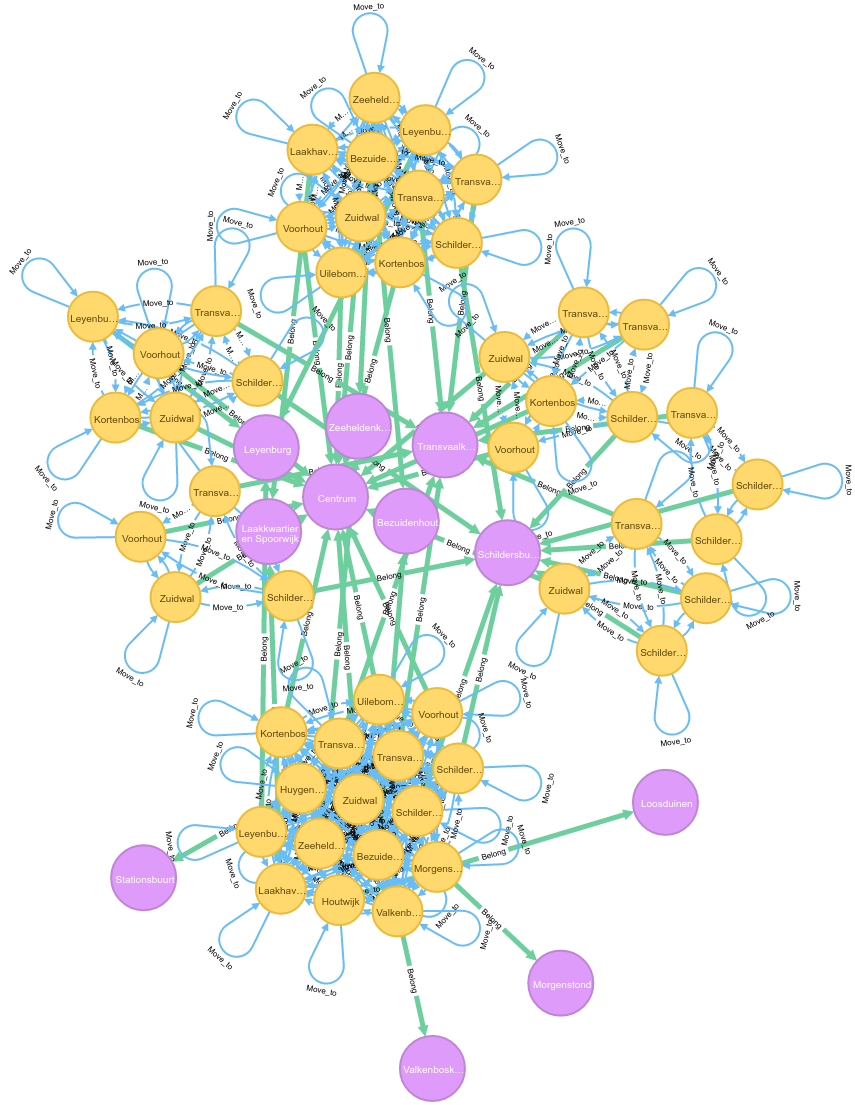
\includegraphics[width=9.5cm]{topcrime_belong1.png}
\caption{Colonias con mayor reubicaci\'on, crimen y criminales: Top 10}
\label{tab:reu_cri_crim}
\end{figure}

Intuitivamente, se infiere que la delincuencia tiende a concentrarse en el centro de las ciudades por las oportunidades que estas representan para los criminales (cantidad de personas, mercanc\'ia, entre otras), esta premisa se corrobor\'o en el grafo analizado.

Es por ello entonces que se dispuso a ordenar por el tipo de arista $flujo$ (tabla 8) y de esta manera visualizar cuales son los caminos cr\'iticos por donde se lleva a cabo la migraci\'on interna.

\begin{table}[H]
\centering
\caption{\textbf{Colonias con mayor reubicaci\'on}}
\scriptsize
\label{top10_fcc}
\begin{tabular}{p{.6cm} p{.5cm} p{1.5cm}| p{.6cm} p{.5cm} p{1.5cm} |p{.8cm}} 
\multicolumn{3}{l}{\textbf{Origen}}                    & \multicolumn{3}{l}{\textbf{Destino}}                   & \textbf{Relaci\'on} \\
\textbf{Criminal} & \textbf{Crimen} & \textbf{Colonia}                 & \textbf{Criminal} & \textbf{Crimen} & \textbf{Colonia}                 & \textbf{Flujos }  \\
\hline
\hline
20         & 79     & Kerketuinen/ Zichtenburg & 374        & 296    & Rond de Energiecentrale & 482      \\
190        & 1216   & Transvaalkwartier-Zuid  & 416        & 1170   & Schildersbuurt-West     & 231      \\
542        & 920    & Schildersbuurt-West     & 217        & 977    & Transvaalkwartier-Zuid  & 203      \\
234        & 774    & Transvaalkwartier-Zuid  & 531        & 842    & Schildersbuurt-West     & 177      \\
286        & 722    & Schildersbuurt-Noord    & 416        & 1170   & Schildersbuurt-West     & 174      \\
531        & 842    & Schildersbuurt-West     & 376        & 543    & Schildersbuurt-Noord    & 160      \\
238        & 727    & Transvaalkwartier-Zuid  & 581        & 856    & Schildersbuurt-West     & 154      \\
223        & 905    & Transvaalkwartier-Zuid  & 488        & 971    & Schildersbuurt-West     & 145      \\
416        & 1170   & Schildersbuurt-West     & 286        & 722    & Schildersbuurt-Noord    & 142      \\
464        & 3586   & Schildersbuurt-West     & 365        & 1024   & Schildersbuurt-Noord    & 140     
\end{tabular}
\end{table}

Resulta que la zona $Kerketuinen/Zichtenburg$ es la que mayor movimiento tiene, es decir que la arista es m\'as pesada con respecto a las dem\'as, aunque en terminos generales no podr\'iamos presumir de un patr\'on con respecto a la evaci\'on de la criminalidad. Adicionalmente a dicha colonia se le aplic\'o el algoritmo Dijkstra y encontrar sus caminos m\'as cortos. Podemos notarlo en la figura 3

\begin{figure}[h]
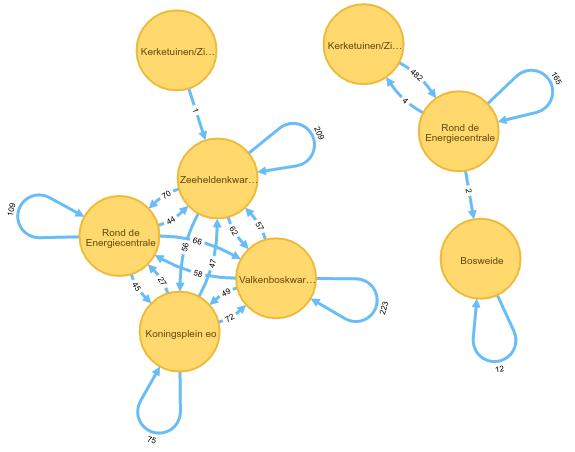
\includegraphics[width=9.5cm]{dijkstra.png}
\caption{Rutas de reubicaci\'on de la colonia con mayor peso}
\end{figure}

\section{DISCUSI\'ON}
\vspace{2mm}
El an\'alisis realizado puede ser extendido de manera importante, ya que con los razonamientos anal\'iticos mostrados, se encontraron notables indicios sobre la migraci\'on interna de la ciudad, como \'areas de oportunidad se podr\'ia considerar, utilizar los nodos tipo a\~no para categorizar propiedades en las relaciones, comparar tambi\'en el movimiento nominal entre distritos, o en todo caso aplicar tambi\'en el algoritmo Dijkstra en variables externas como atracciones o edad de las personas en movimiento.

Es un problema muy interesante, ya que tiene los elementos necesarios para generalizarse, es decir medir la migraci\'on entre ciudades, estados o incluso paises, y encontrar as\'i los caminos cr\'iticos por donde se llevan a cabo los movimientos demogr\'aficos.



%%%%%%%%%%%%%%%%%%%%%%%%%%%%%%%%%%%%%%%%%%%%%%%%%%%%%%%%%%%%%%%%%%%%%%%%%%%%%%%%
\section*{ANEXOS}

Appendixes should appear before the acknowledgment.



%%%%%%%%%%%%%%%%%%%%%%%%%%%%%%%%%%%%%%%%%%%%%%%%%%%%%%%%%%%%%%%%%%%%%%%%%%%%%%%%




\begin{thebibliography}{10}

\bibitem{c1} Daron Acemoglu and Asu Ozdaglar, Graph Theory and Social Networks, Lecture 2, MIT, September 14, 2009.
\bibitem{c2} John Adrian Bondy, Graph Theory with Applications.	Mathermathics: Amsterdam, 1976.
\bibitem{c3} Sonal Raj, Neo4j High Performance.	Packt Publishing, March 2015.
\end{thebibliography}




\end{document}
